\documentclass[12pt]{extarticle}
\usepackage[left = 2cm, right = 2cm, top = 2cm, bottom = 2cm]{geometry}
\usepackage{graphicx}
\usepackage{amsmath}
\usepackage{amssymb}
\usepackage{hyperref}
\usepackage{listings}
\usepackage{caption}
\usepackage{subcaption}
\usepackage{multirow}
\usepackage{bm}
\usepackage{float}
\usepackage{placeins}
\usepackage{pdfpages}
\usepackage{stackengine}
\newcommand\xrowht[2][0]{\addstackgap[.5\dimexpr#2\relax]{\vphantom{#1}}}
\usepackage{diagbox}

\begin{document}

\begin{flushleft}
\begin{LARGE}
\textbf{23.5}
\end{LARGE}  
\end{flushleft}

\vfill
\begin{center}
\begin{Huge}
Ionization of the Interstellar Gas near a Star
\end{Huge}
\end{center}
\vfill

\pagebreak

\begin{center}
\textbf{Question 1}
\end{center}

Integrating over all frequencies and making the substitution $z =\frac{h \nu}{k T_{\star}}$
$$L = \int_0^{\infty} L_{\nu} \,\mathrm{d}\nu  = 4\pi R^2 \frac{2\pi h}{c^2}\int_0^{\infty} \frac{\nu^3}{\exp(\frac{h \nu}{k T_{\star}})-1} \,\mathrm{d}\nu = \frac{8\pi^2 h R^2}{c^2}\left(\frac{kT_{\star}}{h}\right)^4\int_0^{\infty} \frac{z^3}{e^z-1} \,\mathrm{d}z$$

We evaluate the integral using a series expansion for the denominator, which is valid since $0<e^{-z}<1$ for $0<z<\infty$

$$\int_0^{\infty} \frac{z^3}{e^z-1} \,\mathrm{d}z = \int_0^{\infty} \frac{z^3 e^{-z}}{1-e^{-z}} \,\mathrm{d}z = \int_0^{\infty} z^3 e^{-z}\sum_{m = 0}^{\infty} e^{-mz} \,\mathrm{d}z = \sum_{m = 1}^{\infty}\int_0^{\infty} z^3 e^{-mz}\,\mathrm{d}z$$

$$ = \sum_{m = 1}^{\infty}\frac{1}{m^4}\int_0^{\infty} x^3 e^{-x}\,\mathrm{d}x = \Gamma(4)\sum_{m = 1}^{\infty}\frac{1}{m^4} = 6\, \zeta(4) = \frac{\pi^4}{15}$$

where we have made use of $\zeta(4) = \pi^2/90$, which can be shown by considering the Fourier series for $f(x) = x^4$, and the value of $\Gamma(4)$. Combining these we obtain

$$L = \frac{8\pi^6 k^4}{15 c^2 h^3}R^2T_{\star}^4$$

We apply this relation to a few examples.
\begin{itemize}
\item[-] The sun has radius $R = 6.96 \times 10^8$ metres and total luminosity $L = 3.90 \times 10^{26} \mathrm{W}$. Its surface temperature $T_{\star}$ is 
$$T_{\star} = \left(\frac{15c^2 h^3}{8\pi^6 k^4}L R^{-2} \right)^{1/4} = 5796.25 \ldots\, \mathrm{K} \approx 5800 \,\mathrm{K}$$
\item[-] A 7 solar mass star has a surface temperature $T_{\star} = 20,000\,\mathrm{K}$ and a luminosity $L = 4.0 \times 10^{29} \,\mathrm{W}$. Its radius is
$$R= \left(\frac{15c^2 h^3}{8\pi^6 k^4}L T_{\star}^{-4} \right)^{1/2} = 1.8721 \ldots \times 10^9 \,\mathrm{m} \approx 1.9 \times 10^9 \,\mathrm{m}$$
\item[-] A 12 solar mass star has a surface temperature $T_{\star} = 25,000\,\mathrm{K}$ and a luminosity $L = 4.0 \times 10^{30} \,\mathrm{W}$. Its radius is
$$R= \left(\frac{15c^2 h^3}{8\pi^6 k^4}L T_{\star}^{-4} \right)^{1/2} =3.7889  \ldots \times 10^9 \,\mathrm{m} \approx 3.8 \times 10^9 \,\mathrm{m}$$
\end{itemize}

\begin{center}
\textbf{Question 2}
\end{center}

\textbf{Rescaling.} The coefficients involved here have large powers of 10. We rescale the units of measurement to help the compiler in the calculations. Define the new units
$$\mathrm{M} = 10^{-3}\,\mathrm{m}\;\;\;\; \mathrm{S} = 10^{-15}\,\mathrm{s}\;\;\;\; \mathrm{KG} = 10^{-43}\,\mathrm{kg}\;\;\;\; \mathrm{KL} = 10^{4}\,\mathrm{K}$$ 

The coefficients become
$$c = 2.998 \times 10^{-4}\,\mathrm{M\,S^{-1}}\;\;\;\;h = 6.626\,\mathrm{KG\,M^2\,S^{-1}}\;\;\;\;k = 1.381\,\mathrm{KG\,M^2\,S^{-2}\,KL^{-1}}$$
$$a_{\nu_0} = 6.3 \times 10^{-16}\,\mathrm{M^2}\;\;\;\;\nu_0 = 3.29\, \mathrm{S^{-1}}\;\;\;\;\ n_H= 10^{-3}\,\mathrm{M^{-3}}\;\;\;\;\alpha_B (1 \,\mathrm{KL}) = 2.59 \times 10^{-25}\,\mathrm{M^3\,S^{-1}}$$

\textbf{Optical Depth}. The variable $\tau_{\nu_0}$ is a measure of the proportion of the radiation that has been attenuated and is dimensionless. It can be used as the radial coordinate to eliminate the scale of the problem, which can be useful in comparing scenarios of different natures. It is also a monotonically increasing function of the radius.\\

\textbf{Program.} Combining the ionization balance equation with the subsidiary equations gives
$$(n_H-n_p)\left[\frac{2\pi\,\nu_0^3\,a_{\nu_0}\,R^2}{c^2\,r^2}\int_{\nu_0}^\infty \frac{1}{\nu(\exp(\frac{h \nu}{k T_{\star}})-1)}\exp\left(-\tau_{\nu_0}\left(\frac{\nu_0}{\nu}\right)^3\right)\mathrm{d}\nu\right] = n_p^2\alpha_B(T)$$

We continue by making the problem discrete. At each iteration, the built-in integral function on Matlab is used to compute the integral above, giving the quadratic equation
$$(n_p^{(i)})^2+C^{(i)}n_p^{(i)}-n_H C^{(i)} = 0$$

Initially the constants $C^{(i)}$ are too large (or order $10^{17}$) for the quadratic formula to yield the solution accurately. We remedy this by expanding the square root to to order $O(n_H^3)$ to give $n_p^{(i)}$, which also immediately gives $n_{H^0}^{(i)}$. It is left to solve the ODE for $\tau_{\nu_0}^{(i)}$, which we do by employing the Adams-Bashforth method of order 5.\\
 
\begin{center}
\textbf{Question 3}
\end{center}

The ionized and neutral fractions were computed for all nine cases (three stellar masses and three gas temperatures). The plots are shown in figures 1 - 3. In each case we see a sharp transition from the gas being mostly ionized to mostly neutral at some radial distance $r_1$, the values of which are given in table 1 to 2 s.f.. We are able to comment on the different factors affecting the densities.
\begin{itemize}
\item[-]\textbf{Gas Temperature.} In all three cases we see that increasing the temperature extends the region of ionized hydrogen. An increase in the kinetic energy of the particles makes recombination more difficult. This is also apparent in the decrease in the value of $\alpha_B$. Since the distribution of photons is unaffected  it is expected that the radius of ionization would indeed increase with temperature.
\item[-]\textbf{Surface Temperature.} An increase in the surface temperature of the star affects the distribution of the radiation flux by increasing its height as well as by skewing it to the right; there is more radiation and it is composed of higher frequencies. We expect this to increase the size of the ionized region, which is indeed what we see by comparing the plots for the three stars.
\item[-]
\textbf{Radius of Star.} A greater star radius increases the luminosity. More photons are emitted per second and therefore more hydrogen atoms are ionized, extending the region of ionization.\\
\end{itemize}

\begin{center}
\textbf{Question 4}
\end{center}

We integrate the ionization balance equation over $r$ from $0$ to $\infty$ and make the approximation $n_p = n_e = n_H$ for $r\leq r_1$ and $n_p=n_e = 0$ for $r>r_1$, which seems appropriate by looking at the plots.  
$$\int_{\nu_0}^{\infty}\frac{L_{\nu}}{h\nu}\left[\int_0^{\infty}n_{H^0}a_{\nu}e^{-\tau_{\nu}}\mathrm{d}r\right]\mathrm{d}\nu = \int_0^{r_1}4\pi r^2 n_H^2 \alpha_B(T)\,\mathrm{d}r$$

From the definition of $\tau_{\nu}$ we have $\mathrm{d}\tau_{\nu}  = n_{H^0}a_{\nu}\mathrm{d}r$. We approximate $\tau_{\nu}(0) = 0$ by treating the star as a point mass. For the upper limit, $\tau_{\nu} \rightarrow  \infty$ as $r \rightarrow \infty$ since $\tau_{\nu}(r)$ is a strictly increasing function. Making the substitution yields

$$\int_{\nu_0}^{\infty}\frac{L_{\nu}}{h\nu}\left[\int_0^{\infty}e^{-\tau_{\nu}}\mathrm{d}\tau_{\nu}\right]\mathrm{d}\nu = \frac{4\pi}{3} r_1^3 n_H^2 \alpha_B$$
 
$$Q(H) \equiv \int_{\nu_0}^{\infty}\frac{L_{\nu}}{h\nu}\mathrm{d}\nu = \frac{4\pi}{3} r_1^3 n_H^2 \alpha_B$$ 

The total energy emitted per second carried by photons of frequency $\nu$ is $L_{\nu}$. Since each such photon has energy $h\nu$, the total number of photons of this frequency is $L_{\nu}/h\nu$. Only photons of frequency greater than $\nu_0$ are ionizing. Integrating over this quantity gives the total number of ionizing photons, which is indeed $Q(H)$. Substituting for $L_{\nu}$ gives
$$Q(H) = \frac{8\pi^2 R^2}{c^2} \int_{\nu_0}^\infty \frac{\nu^2}{\exp(\frac{h \nu}{k T_{\star}})-1}\mathrm{d}\nu$$

Values of $Q(H)$ are shown for the cases above in table 2. Rearranging for $r_1$ gives
$$r_1 = \left[\frac{3Q(H)}{4\pi n_H^2\alpha_B}\right]^{1/3}$$

We use this expression to find approximations to $r_1$, shown in table 3. We compare the two sets of values for $T = 10,000$K. The values for the Sun differ but are of the same order of magnitude; from the plot we see the transition is fairly smooth, making the approximation slightly crude. The values for the other stars are in good agreement. The transitions are much sharper so the approximation is more suitable for these. \\

\begin{center}
\textbf{Question 5}
\end{center}

The proportions of the ionized and neutral hydrogen densities were computed for the quasar. Values of the neutral hydrogen density are shown in table 4. Both densities were plotted and are shown in figure 4.\\

The galaxy has radius $3\times 10^{20}$m. We observe that none of the interstellar gas in the galaxy has neutral fraction greater than 0.5. Indeed almost all the interstellar gas in the galaxy is ionized.\\

Following the same calculations as in question 4 we find that $Q(H) = 8.5 \times 10^{56}$ - that's a lot of photons! From this we find the approximate value of $r_1$ is $9.2\times 10^{20}$, in good agreement with the plots.

\pagebreak

\begin{center}
\textbf{Tables and Figures}
\end{center}


\begin{table}[!htbp]
\centering
\begin{tabular}{|c||c|c|c|}
\hline \xrowht{35pt}
Temperature (K)& \;\;\;\;5,000\;\;\;\; & \;\;\;10,000\;\;\; & \;\;\;20,000\;\;\; \\
\hline \hline\xrowht{35pt}
Sun ($10^{13}$ m)& 1.3 & 1.8 & 1.8 \\
\hline\xrowht{35pt}
7 Solar mass ($10^{17}$ m) & 1.6 & 2.0 & 2.0  \\ 
\hline\xrowht{35pt}
12 Solar mass ($10^{17}$ m) & 4.7 & 5.7 & 5.7 \\ 
\hline
\end{tabular}
\caption{The values of $r_1$ obtained from the plots}
\label{Table:1}
\end{table}

\begin{table}[!htbp]
\centering
\begin{tabular}{|c||c|c|c|}
\hline \xrowht{35pt}
Star & \hspace{7mm} Sun \hspace{7mm} & \hspace{2mm}7 Solar mass\hspace{2mm} &12 Solar mass \\
\hline \xrowht{35pt}
\;\;\;\;$Q(H)$\;\;\;\; & $9.1\times 10^{35}$ & $6.9\times 10^{45}$& $1.8\times 10^{47}$  \\
\hline
\end{tabular}
\caption{The values of $Q(H)$}
\label{Table:2}
\end{table}


\begin{table}[!htbp]
\centering
\begin{tabular}{|c||c|c|c|}
\hline \xrowht{35pt}
Temperature (K)& \;\;\;\;5,000\;\;\;\; & \;\;\;10,000\;\;\; & \;\;\;20,000\;\;\; \\
\hline \hline\xrowht{35pt}
Sun ($10^{13}$ m)& 7.8 & 9.4 & 9.5 \\
\hline\xrowht{35pt}
7 Solar mass ($10^{17}$ m) & 1.5 & 1.9 & 1.9  \\ 
\hline\xrowht{35pt}
12 Solar mass ($10^{17}$ m) & 4.5 & 5.5 & 5.5 \\ 
\hline
\end{tabular}
\caption{The approximated values of $r_1$}
\label{Table:3}
\end{table}

\begin{table}[!htbp]
\begin{center}
\begin{tabular}{|c|c|}
\hline\xrowht{20pt}
Radius ($10^{20}$m)& Neutral Hydrogen\\
\hline \hline\xrowht{10pt}
1 & 0.000000 \\ \xrowht{15pt} 
2 & 0.000001 \\ \xrowht{15pt} 
3 & 0.000002 \\ \xrowht{15pt} 
4 & 0.000003 \\ \xrowht{15pt} 
5 & 0.000006 \\ \xrowht{15pt} 
6 & 0.000011 \\ \xrowht{15pt} 
7 & 0.000025 \\ \xrowht{15pt} 
8 & 0.000106 \\ \xrowht{15pt} 
9 & 0.007505 \\ \xrowht{15pt} 
10 & 0.977304 \\ \xrowht{15pt} 
11 & 0.993158 \\ \xrowht{15pt} 
12 & 0.996686 \\ \xrowht{15pt} 
13 & 0.998068 \\ \xrowht{15pt} 
14 & 0.998753 \\ \xrowht{15pt} 
15 & 0.999140 \\ \xrowht{15pt} 
16 & 0.999378 \\ \xrowht{15pt} 
17 & 0.999534 \\ \xrowht{15pt} 
18 & 0.999642 \\ \xrowht{15pt} 
19 & 0.999718 \\ \xrowht{15pt} 
20 & 0.999774 \\ 
\hline
\end{tabular}
\quad
\begin{tabular}{|c|c|}
\hline\xrowht{20pt}
Radius ($10^{20}$m)& Neutral Hydrogen\\
\hline \hline \xrowht{10pt}
8.0 & 0.000106 \\ \xrowht{15pt} 
8.1 & 0.000132 \\ \xrowht{15pt} 
8.2 & 0.000168 \\ \xrowht{15pt} 
8.3 & 0.000218 \\ \xrowht{15pt} 
8.4 & 0.000293 \\ \xrowht{15pt} 
8.5 & 0.000408 \\ \xrowht{15pt} 
8.6 & 0.000597 \\ \xrowht{15pt} 
8.7 & 0.000929 \\ \xrowht{15pt} 
8.8 & 0.001580 \\ \xrowht{15pt} 
8.9 & 0.003074 \\ \xrowht{15pt} 
9.0 & 0.007505 \\ \xrowht{15pt} 
9.1 & 0.028704 \\ \xrowht{15pt} 
9.2 & 0.241903 \\ \xrowht{15pt} 
9.3 & 0.714505 \\ \xrowht{15pt} 
9.4 & 0.863825 \\ \xrowht{15pt} 
9.5 & 0.916885 \\ \xrowht{15pt} 
9.6 & 0.942394 \\ \xrowht{15pt} 
9.7 & 0.956994 \\ \xrowht{15pt} 
9.8 & 0.966305 \\ \xrowht{15pt} 
9.9 & 0.972690 \\
\hline
\end{tabular}\vspace{10mm}
\caption{The neutral hydrogen density. The table on the right shows the transition in more detail.}
\end{center}
\end{table}

\begin{figure}[h]
    \centering
    \begin{subfigure}[b]{0.53\textwidth}
        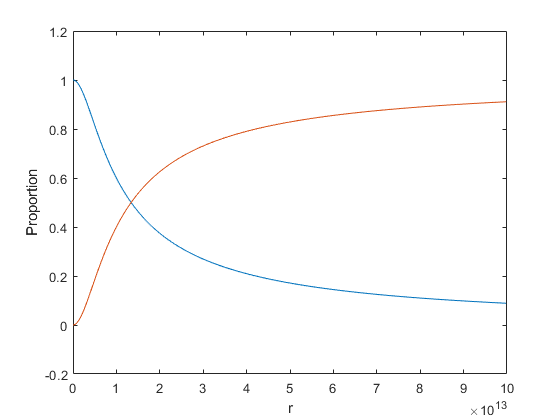
\includegraphics[width=\textwidth]{Sun_5.png}
        \caption{$T$ = 5,000K}
        \label{figure:1a}
    \end{subfigure}  
    \qquad
    \begin{subfigure}[b]{0.53\textwidth}
        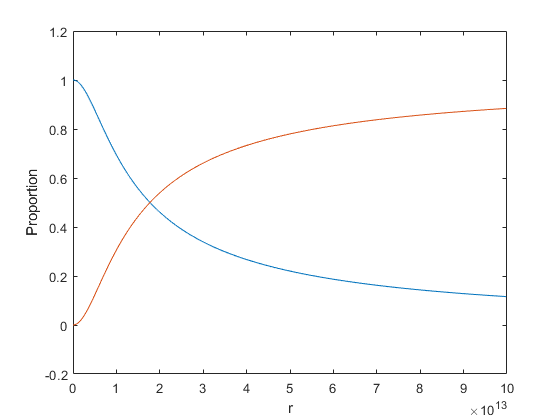
\includegraphics[width=\textwidth]{Sun_10.png}
        \caption{$T$ = 10,000K}
        \label{figure:1b}
    \end{subfigure} 
    \\ 
    \begin{subfigure}[b]{0.53\textwidth}
        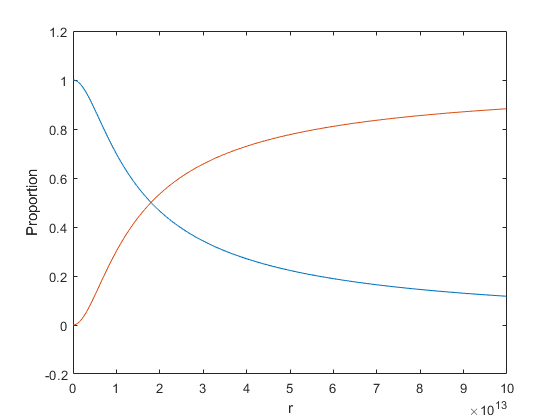
\includegraphics[width=\textwidth]{Sun_20.png}
        \caption{$T$ = 20,000K}
        \label{figure:1c}
    \end{subfigure} 
    \caption{Plots of the ionization and neutral fractions for the Sun}\label{figure 1}
\end{figure}

\begin{figure}[h]
    \centering
    \begin{subfigure}[b]{0.53\textwidth}
        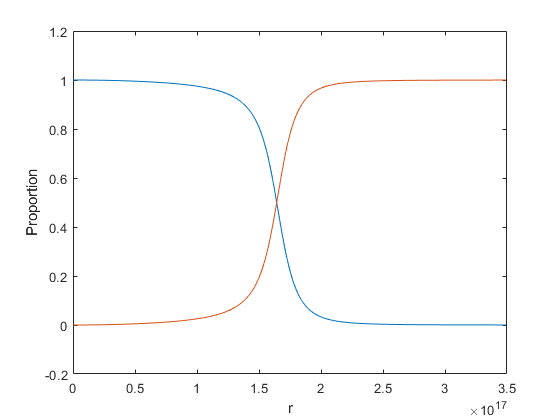
\includegraphics[width=\textwidth]{7_5.png}
        \caption{$T$ = 5,000K}
        \label{figure:2a}
    \end{subfigure}  
    \qquad
    \begin{subfigure}[b]{0.53\textwidth}
        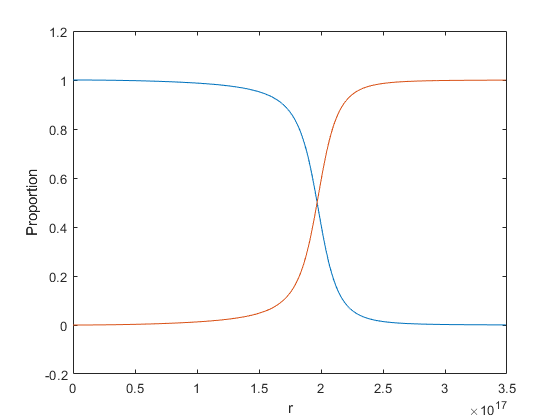
\includegraphics[width=\textwidth]{7_10.png}
        \caption{$T$ = 10,000K}
        \label{figure:2b}
    \end{subfigure} 
    \\ 
    \begin{subfigure}[b]{0.53\textwidth}
        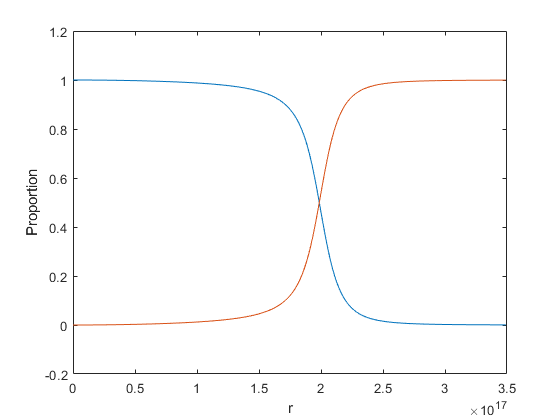
\includegraphics[width=\textwidth]{7_20.png}
        \caption{$T$ = 20,000K}
        \label{figure:2c}
    \end{subfigure} 
    \caption{Plots of the ionization and neutral fractions for the 7 solar mass star}\label{figure 2}
\end{figure}

\begin{figure}[h]
    \centering
    \begin{subfigure}[b]{0.53\textwidth}
        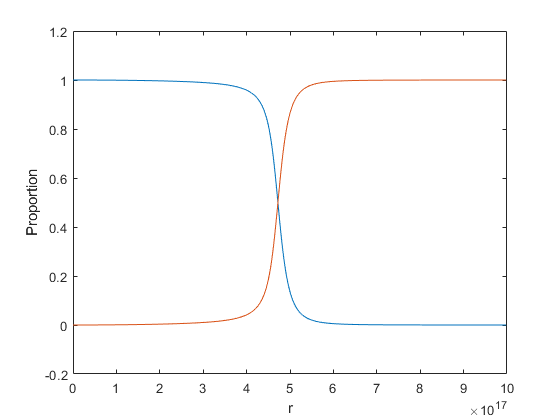
\includegraphics[width=\textwidth]{12_5.png}
        \caption{$T$ = 5,000K}
        \label{figure:3a}
    \end{subfigure}  
    \qquad
    \begin{subfigure}[b]{0.53\textwidth}
        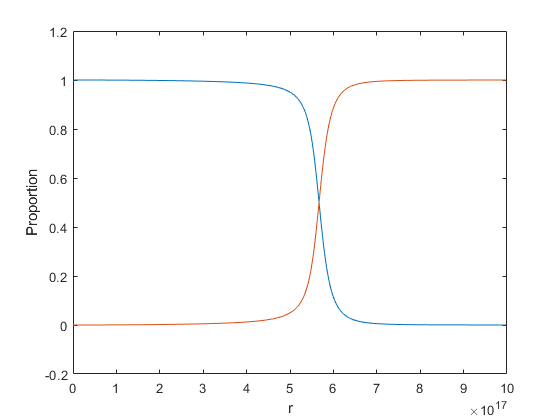
\includegraphics[width=\textwidth]{12_10.png}
        \caption{$T$ = 10,000K}
        \label{figure:3b}
    \end{subfigure} 
    \\ 
    \begin{subfigure}[b]{0.53\textwidth}
        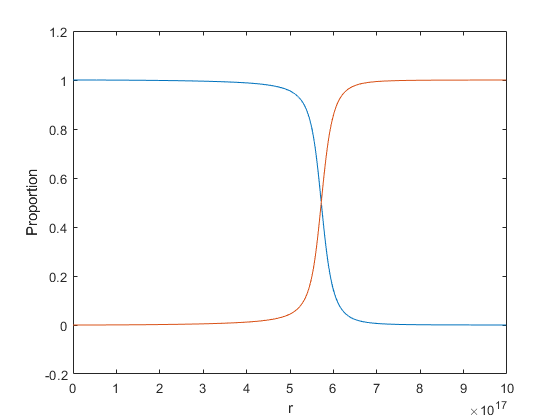
\includegraphics[width=\textwidth]{12_20.png}
        \caption{$T$ = 20,000K}
        \label{figure:3c}
    \end{subfigure} 
    \caption{Plots of the ionization and neutral fractions for the 12 solar mass star}\label{figure 3}
\end{figure}

\begin{figure}[h]
    \centering
    \begin{subfigure}[b]{0.6\textwidth}
        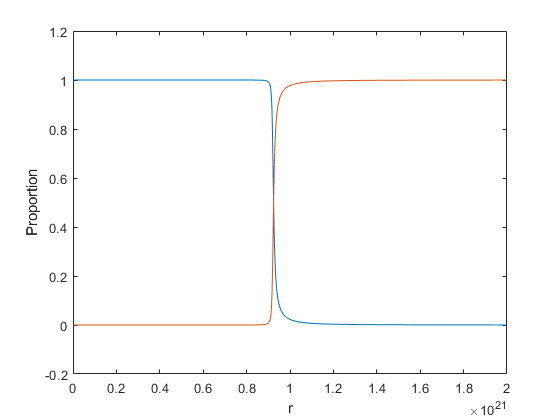
\includegraphics[width=\textwidth]{Quasar.png}
		\caption{Large range behaviour}
        \label{figure:4a}
    \end{subfigure}  
    \qquad
    \begin{subfigure}[b]{0.6\textwidth}
        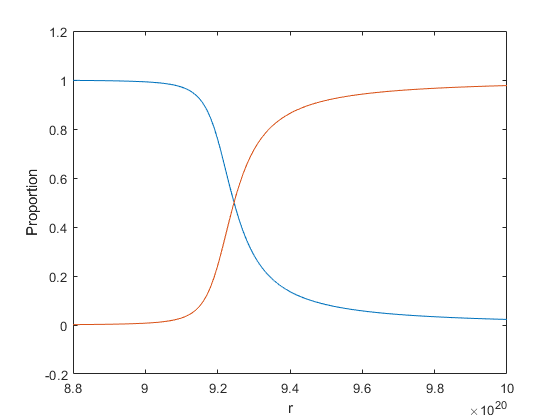
\includegraphics[width=\textwidth]{QuasarClose.png}
        \caption{The transition in more detail}
        \label{figure:4b}
    \end{subfigure} 
    \caption{Plots of the ionization and neutral fractions for the quasar} 
    \label{figure 4}
\end{figure}

    
\pagebreak
\FloatBarrier
\begin{center}
\textbf{Code Listings}
\end{center}

\begin{center}
Solution of the ionization equations
\end{center}
\lstinputlisting[language=Matlab]{Solution.m}

\begin{center}
Question 4
\end{center}
\lstinputlisting[language=Matlab]{Question4.m}

\begin{center}
Integral for Stars
\end{center}
\lstinputlisting[language=Matlab]{Int.m}

\begin{center}
Integral for Quasar
\end{center}
\lstinputlisting[language=Matlab]{QInt.m}

\end{document}

